\documentclass[fontset=windows]{article}
\usepackage[]{ctex}
\usepackage[a4paper, total={6in, 8in}]{geometry}

\title{LSM-KV 项目报告}
\author{池昊 522031910095}
\date{2024年 5月 29日}

\usepackage{natbib}
\usepackage{graphicx}
\usepackage{enumitem}
\usepackage{booktabs}
\bibliographystyle{plain}

\begin{document}

\maketitle

\section{背景介绍}
LSM树(Log-Structured Merge-Tree)是一种专为写密集型应用设计的数据结构,常用于实现键值存储系统。与传统的平衡树结构(如B树)相比,LSM树通过减少对磁盘的写操作次数和优化写入路径来提高写入性能。LSM树主要由两部分组成:内存中的数据结构(通常是跳表或者红黑树)和硬盘上的多个有序的不可变文件。该项目增加了Vlog文件用于储存键值,SSTable中不再储存值,而是储存键对应的值在Vlog文件中的偏移量,从而实现了键值分离的LSM树。本实验通过正确性测试和持久性测试验证了实现的正确性,并通过一系列性能测试验证其操作性能。

\section{测试}

\subsection{性能测试}

\subsubsection{预期结果}

\begin{enumerate}
    \item 常规分析:\par
    对于Get、Put、Delete、Scan这四种操作,我们预期随着数据大小的增加,操作的延迟也将增加。这种延迟增加主要由于数据量增大导致操作访问SSTable数量增加,相应IO操作和Compaction操作数量增加。我们将通过对不同数据大小执行这些操作并计算平均延迟来验证这一预期。并且吞吐量会相应减小。

    \item 索引缓存与Bloom Filter的效果测试:
    \begin{enumerate}
        \item 在没有任何缓存的情况下,预期GET操作将展示较高的延迟,因为每次操作都需要从磁盘中检索数据。
        \item 当索引信息被缓存时,由于减少了对磁盘的访问,预期GET操作的延迟将有显著降低。
        \item 当添加Bloom Filter后,预期在存在大量非目标数据的查询时,GET操作的延迟将进一步减少,因为Bloom Filter可以有效减少不必要的SSTable访问。
    \end{enumerate}

    \item Compaction的影响:\par
    随着数据的持续写入,系统将定期执行Compaction操作。预期在Compaction执行期间,系统的PUT请求处理吞吐量将受到影响,具体表现为吞吐量的下降。

    \item Bloom Filter大小配置的影响:\par
    通过设置不同大小的Bloom Filter并保持SSTable大小不变,预期可以观察到Bloom Filter大小对Get和Put操作性能的具体影响。一个过大的Bloom Filter可能会导致频繁的SSTable合并,而过小的Bloom Filter可能导致较高的误判率。这将帮助确定最优的Bloom Filter大小,以平衡性能和资源使用。
\end{enumerate}

\subsubsection{常规分析}
该测试中,分别测试了键的数量在512,12K及48K三种情况下Get、Put、Delete、Scan操作的平均延迟和吞吐量。为了避免磁盘IO操作对延迟的影响,将插入Value大小固定为64个字节。得到结果如表~\ref{tab:regular_latency}和表~\ref{tab:regular_throughput}所示。

\begin{table}[ht]
    \centering
    \begin{tabular}{ccccc}
        \toprule
        \textbf{键数量} & \textbf{Get} & \textbf{Put} & \textbf{Delete} & \textbf{Scan} \\
        \midrule
        512 & 6.007 & 2.815 & 7.471 & 1050.85 \\
        12K & 13.099 & 14.490 & 23.666 & 249275 \\
        48K & 16.967 & 30.996 & 65.308 & 2397400 \\
        \bottomrule
    \end{tabular}
    \caption{常规测试中操作平均延迟(ms)}
    \label{tab:regular_latency}
\end{table}

由结果可得,各操作随键数量增加均表现出平均延迟增大,吞吐量减小的情况。

\begin{table}[ht]
    \centering
    \begin{tabular}{ccccc}
        \toprule
        \textbf{键数量} & \textbf{Get} & \textbf{Put} & \textbf{Delete} & \textbf{Scan} \\
        \midrule
        512 & 166480 & 355244 & 133859 & 951.61 \\
        12K & 76340.3 & 69012.6 & 42254.6 & 4.01164 \\
        48K & 58938.7 & 32262.4 & 15312.1 & 0.417118 \\
        \bottomrule
    \end{tabular}
    \caption{常规测试中操作吞吐量(ops/sec)}
    \label{tab:regular_throughput}
\end{table}

\subsubsection{索引缓存与Bloom Filter的效果测试}
该测试中测试了在键数量为12K时,在以下三种缓存策略下Get操作的平均时延和吞吐量:
\begin{enumerate}
    \item 内存中没有缓存SSTable的任何信息,从磁盘中访问SSTable的索引,在找到offset之后读取数据
    \item 内存中只缓存了SSTable的索引信息,通过二分查找从SSTable的索引中找到offset,并在磁盘中读取对应的值
    \item 内存中缓存SSTable的Bloom Filter和索引,先通过Bloom Filter判断一个键值是否可能在一个SSTable中,如果存在再利用二分查找,否则直接查看下一个SSTable的索引
\end{enumerate}
结果如表~\ref{tab:cache_test}所示

\begin{table}[ht]
    \centering
    \begin{tabular}{ccc}
        \toprule
        \textbf{缓存策略} & \textbf{平均时延(ms)} & \textbf{吞吐量(ops/sec)} \\
        \midrule
        全缓存 & 41.356 & 24180 \\
        只缓存索引 & 46.019 & 51648.3 \\
        无缓存 & 3969.5 & 251.92 \\
        \bottomrule
    \end{tabular}
    \caption{不同缓存策略下GET操作平均时延和吞吐量}
    \label{tab:cache_test}
\end{table}

由结果可得,无缓存策略由于频繁的读写操作会严重影响GET操作的性能。使用Bloom Filter也可以进一步提高性能,但是可能由于Bloom Filter实现导致值检验性能不高,其优势并不明显。

\subsubsection{Compaction的影响}
该测试中记录了不断插入数据的情况下,每一次操作的平均时延,绘制折线图如图~\ref{fig:compaction_test}所示。 \par

\begin{figure}[ht!]
    \centering
    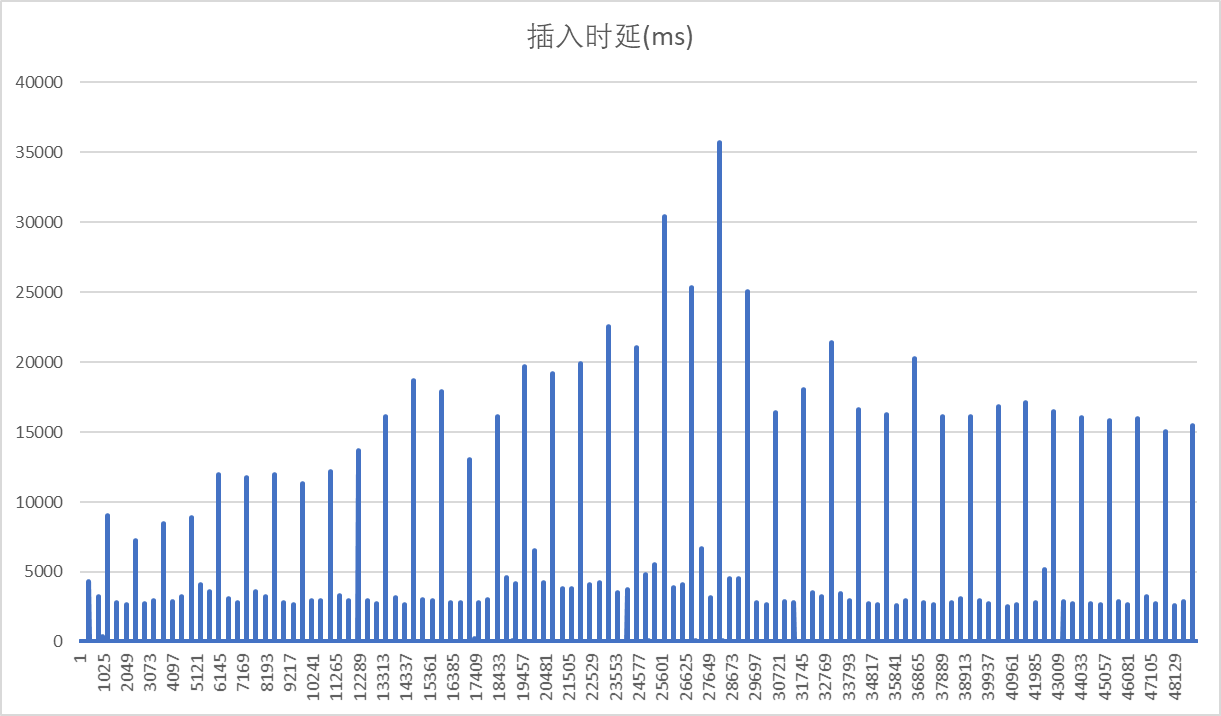
\includegraphics[width=0.9\textwidth]{compaction_test.png}
    \caption{插入操作时延(ms)}
    \label{fig:compaction_test}
\end{figure}

由于每一个SSTable在给定的SSTable和Bloom Filter大小下最多能储存408个数据,并且在第一层SSTable数量为3时触发一次Compaction,即每插入1224个数据会触发一次Compaction。由折线图可以看出,在每一次键值为1224倍数时有一次明显的峰值。因为本实验中PUT操作的实现包含了SSTable写入磁盘的操作,在数据量为408的倍数时,Latency由于IO操作也会出现峰值。但没有触发Compaction时时延大。

\subsubsection{Bloom Filter 大小配置的影响}
该测试中测试了在键数量为48K时,在不同Bloom Filter大小下得到的PUT和GET操作吞吐量,结果如表~\ref{tab:bloom_filter_test}

\begin{table}[ht]
    \centering
    \begin{tabular}{ccc}
        \toprule
        \textbf{Bloom Filter大小} & \textbf{Get} & \textbf{Put} \\
        \midrule
        12K & 2403.81 & 5656.57 \\
        10K & 2530.16 & 6172.8 \\
        8K & 2609.35 & 6791.74 \\
        6K & 2550.76 & 6645.34 \\
        4K & 2562.80 & 6962.29 \\
        2K & 2523.77 & 7219.24 \\
        \bottomrule
    \end{tabular}
    \caption{Bloom Filter大小对操作吞吐量(ops/sec)的影响}
    \label{tab:bloom_filter_test}
\end{table}

从实际结果来看PUT操作有随Bloom Filter大小增加,吞吐量先增大后减小的趋势,而GET操作并不明显,在Bloom Filter大小达到最小2K字节时,吞吐量达到最大7219.24ops/sec。这可能是因为Bloom Filter持续减小,虽然假阳性率增大,但被储存键值数量增加带来SSTable数量减少带来的影响所抵消。

\section{结论}
本项目通过一系列的测试验证了基于LSM树的键值存储系统的性能,并探索了不同的优化策略对系统性能的影响,测试结果基本符合预期。通过这些测试,我们可以得出结论,LSM树的实现可以通过适当的优化(如索引缓存和Bloom Filter的使用)显著提高性能。Bloom Filter选择合适的参数也可以提高性能。

\section{致谢}
感谢我的朋友侯明希在我写整个项目过程中叫我出去吃饭,缓解我debug带来的压力。感谢机核网的电台节目,在我写项目焦虑时带来了一点平静。感谢和山山老师的作品《为你着迷》和《女校之星》,在我项目实现的几天的闲暇时间里读完了这两部很好看的漫画。

\section{其他和建议}
在本人的拖延下,在项目发布到第十三周整个项目基本没有怎么推进。从第十四周周一开始才完成第二次迭代的要求,并且第一次通过测试。最后于周四完成了整个项目的代码实现。整个项目实现并没有花费太多时间,也没有遇到很大的困难,但是因为拖延还是给我带来了深深的焦虑感,也几度不是很想写了。最后一个bug是在compaction实现中,把整个结构中最大时间戳当作合并的sstable中最大时间戳赋给了新的sstable,这一愚蠢的bug。在做完所有项目和lab后,忽然想起所有homework、lab和project加起来只有整个课程分数40$\%$的占比。或许三学分和40$\%$并不匹配这门课的workload吧,我不认为减少workload是解决这个问题的最佳途径,或许未来可以调整学分或调整最终对分值比例构成。祝愿软院和ADS课程越办越好。

\end{document}
